\let\negmedspace\undefined
\let\negthickspace\undefined
\documentclass[article]{IEEEtran}
\usepackage[a5paper, margin=10mm, onecolumn]{geometry}
%\usepackage{lmodern} % Ensure lmodern is loaded for pdflatex
\usepackage{tfrupee} % Include tfrupee package

\setlength{\headheight}{1cm} % Set the height of the header box
\setlength{\headsep}{0mm}     % Set the distance between the header box and the top of the text

\usepackage{gvv-book}
\usepackage{gvv}
\usepackage{cite}
\usepackage{amsmath,amssymb,amsfonts,amsthm}
\usepackage{algorithmic}
\usepackage{graphicx}
\usepackage{textcomp}
\usepackage{xcolor}
\usepackage{txfonts}
\usepackage{listings}
\usepackage{enumitem}
\usepackage{mathtools}
\usepackage{gensymb}
\usepackage{comment}
\usepackage[breaklinks=true]{hyperref}
\usepackage{tkz-euclide} 
\usepackage{listings}                                       
\def\inputGnumericTable{}                                 
\usepackage[latin1]{inputenc}                                
\usepackage{color}                                            
\usepackage{array}                                            
\usepackage{longtable}                                       
\usepackage{calc}                                             
\usepackage{multirow}                                         
\usepackage{hhline}                                           
\usepackage{ifthen}                                           
\usepackage{lscape}

\renewcommand{\thefigure}{\theenumi}
\renewcommand{\thetable}{\theenumi}
\setlength{\intextsep}{10pt} % Space between text and floats

\numberwithin{figure}{enumi}
\renewcommand{\thetable}{\theenumi}

% Marks the beginning of the document
\begin{document}
\bibliographystyle{IEEEtran}
\title{NCERT-10.4.ex.15}
\author{EE24BTECH11039 - MANDALA RANJITH}
{\let\newpage\relax\maketitle}


\subsection*{Question}
A motor boat whose speed is 18 km/h in still water takes 1 hour more to go 24 km upstream than to return downstream to the same spot. Find the speed of the stream.

\subsection*{Theoritical Solution}

Let the speed of the stream be  $x$  km/h.

Therefore, the speed of the boat upstream = $ \brak{18 - x}$ km/h and the speed of the boat downstream = $\brak{18 + x}$ km/h.

The time taken to go upstream is:
\begin{align}
\text{Time} = \frac{\text{Distance}}{\text{Speed}} = \frac{24}{18 - x} \text{ hours.}
\end{align}

Similarly, the time taken to go downstream is:
\begin{align}
\frac{24}{18 + x} \text{ hours.}
\end{align}

According to the question,
\begin{align}
\frac{24}{18 - x} - \frac{24}{18 + x} = 1
\end{align}

Multiplying throughout by \( 24(18 + x)(18 - x) \), we get:

\begin{align}
24(18 + x) - 24(18 - x) = (18 - x)(18 + x)
\end{align}

\begin{align}
x^2 + 48x - 324 = 0
\end{align}

Using the quadratic formula:

\begin{align}
x = \frac{-48 \pm \sqrt{48^2 + 1296}}{2} = \frac{-48 \pm \sqrt{3600}}{2}
\end{align}

\begin{align}
= \frac{-48 \pm 60}{2}
\end{align}

\begin{align}
= 6 \text{ or } -54
\end{align}
Since \( x \) is the speed of the stream, it cannot be negative. So, we ignore the root \( x = -54 \). 

Therefore, \( x = 6 \) gives the speed of the stream as \textbf{6 km/h}.

\begin{align}
    \textbf{Theorem: }
\end{align}
    Let $x = s$ be a solution of $x = g\brak{x}$ and suppose that $g$ has a continuous
    derivative in some interval $J$ containing $s$. Then if $\abs{g^{\prime}} \le K < 1$ in $J$,
    the iteration process defined  above converges for any $x_0$ in $J$. The limit of the sequence
    $\sbrak{x_n}$ is s\\
\newline
Since there is no solution (evident by quadratic formula) there exists no interval J for which
the process converges to a point.\\
\newline
The same behaviour is shown by the Newton-Raphson Method,\\
Start with an initial guess $x_0$, and then run the following logical loop,
\begin{align}
    x_{n+1} = x_n - \frac{f\brak{x_n}}{f^{\prime}\brak{x_n}} 
\end{align}
where ,
\begin{align}
    f\brak{x} = x^2 + 48x - 324\\
    f^{\prime}\brak{x} = 2x+48
\end{align}




\textbf{CODING LOGIC FOR FINDING EIGENVALUES :-}\\


The quadratic equation 
\begin{align}
x^2 + 48x - 324 = 0
\end{align}
is rewritten in matrix form:
\begin{align}
\text{Matrix} =
\myvec{0 & -\frac{c}{a} \\
1 & -\frac{b}{a}
}
\end{align}

\begin{align}
a = 1, \quad b = 48, \quad c =-324.
\end{align}

Substituting the values of $a,b$ and $c$, the matrix becomes:\\
Let
\begin{align}
\text{A} =
\myvec{0 & 324 \\
1 & -\frac{48}{1}
}
\end{align}




\textbf{QR-DECOMPOSITION:-GRAM-SCHMIDT METHOD}\\



\begin{enumerate}

\item QR decomposition 
\begin{align}
A = QR
\end{align}
\begin{enumerate}
    \item $Q$ is an $ m \times n $ orthogonal matrix
    \item $R$ is an $n \times n$ upper triangular matrix.
\end{enumerate}
Given a matrix $ A = [a_1, a_2, \dots, a_n] $, where each $ a_i $ is a column vector of size $ m \times 1 $.

\item Normalize the first column of $A$:
\begin{align}
q_1 = \frac{a_1}{\norm{a_1}}
\end{align}

\item  For each subsequent column $ a_i $, subtract the projections of the previously obtained orthonormal vectors from $ a_i $ :
\begin{align}
a_i' = a_i - \sum_{k=1}^{i-1} \langle a_i, q_k \rangle q_k
\end{align}
Normalize the result to obtain the next column of \( Q \):
\begin{align}
q_i = \frac{a_i'}{\norm{a_i'}}
\end{align}

Repeat this process for all columns of \( A \).

\item Finding $R$:- \\
After constructing the ortho-normal columns $ q_1, q_2, \dots, q_n $ of $Q$, we can compute the elements of $R$ by taking the dot product of the original columns of $A$ with the columns of $Q$:

\begin{align}
    r_{ij} = \langle a_j, q_i \rangle \text{ , for  }  i \leq j 
\end{align}
\end{enumerate}



\textbf{QR-Algorithm}\\
\begin{enumerate}
\item Initialization \\
Let $A_0 = A $, where $A$ is the given matrix.

\item QR Decomposition \\
For each iteration $ k = 0, 1, 2, \dots $:
\begin{enumerate}
    \item Compute the QR decomposition of \( A_k \), such that:
    \begin{align}
    A_k = Q_k R_k
    \end{align}
    where:
    \begin{enumerate}
        \item $Q_k $ is an orthogonal matrix ($ Q_k^\top Q_k = I $).
        \item $ R_k $ is an upper triangular matrix.
    \end{enumerate}
    The decomposition ensures $ A_k = Q_k R_k $.

    \item Form the next matrix \( A_{k+1} \) as:
    \begin{align}
    A_{k+1} = R_k Q_k
    \end{align}
\end{enumerate}

\item Convergence\\
Repeat Step 2 until $ A_k $ converges to an upper triangular matrix $ T $. The diagonal entries of $T$ are the eigenvalues of $A$.\\
\item The eigenvalues of matrix will be the roots of the equation.


\end{enumerate}




\begin{figure}[h!]
   \centering
   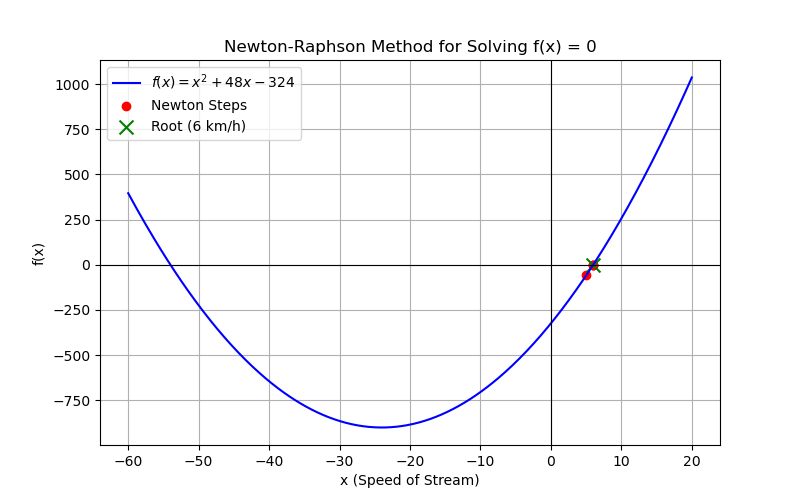
\includegraphics[width=0.8\textwidth]{figures/fig.png} % Ensure this path is correct
   \caption{Plot showing the relationship between $f\brak{x}$ and speed of stream}
   \label{stemplot}
\end{figure}
\end{frame}




\begin{figure}[h!]
   \centering
   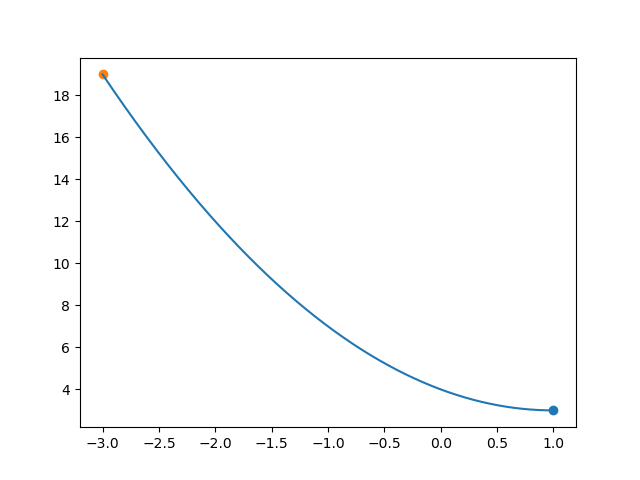
\includegraphics[width=0.8\textwidth]{figures/fig2.png} % Ensure this path is correct
   \caption{Plot showing the relationship between $f\brak{x}$ and speed of stream}
   \label{stemplot}
\end{figure}
\end{frame}



\end{document}


